\documentclass[10pt]{report}
\usepackage{/Users/bradenhoagland/latex/math}

\lhead{Braden Hoagland}
\chead{HW 4}
\rhead{}

\renewcommand{\theenumi}{\alph{enumi}}

\begin{document}
%\tableofcontents

\begin{exer}[DF 14.1: 7.]
	\begin{enumerate}
		\item $\sigma \in \text{Aut}_{\mathbb{Q}}(\mathbb{R})$ takes squares to squares and positive reals to positive reals, and so preserves inequalites.
		\item $\sigma$ is continuous.
		\item Any continuous map on $\mathbb{R}$ which fixes $\mathbb{Q}$ is the identity.
	\end{enumerate}
\end{exer}
\begin{enumerate}
	\item Let $\sigma\in \text{Aut}_{\mathbb{Q}}(\mathbb{R})$, and let $r^2 \in \mathbb{R}$. Since $\sigma$ is a homomorphism, $\sigma(r^2)\sigma(r)^2$, so $\sigma$ maps squares to squares. For all $r \in \mathbb{R}$, $\sqrt{r} $ is also a real number, so every $r$ is a square, so $\sigma$ maps all positive real numbers to positive real numbers.

		Now since $\mathbb{Q}$ is dense in $\mathbb{R}$, for real numbers $a,b$ we can find a rational $q$ such that $a<q<b$. Then $q-a$ and $b-q$ are both positive real numbers. Then because $\sigma$ maps positive reals to positive reals,
		\begin{align*}
			q &= \sigma(q) = \sigma(q-a)+\sigma(a) > \sigma(a), \\
			q &= \sigma(q) = -\sigma(b-q)+\sigma(b) < \sigma(b).
		\end{align*}
		This implies $\sigma(a)<q<\sigma(b)$.

	\item If $a-b < \frac{1}{m} $, then $\sigma(a)-\sigma(b) < \sigma(1/m) = 1/m$, where the last equality follows from $1/m$ being rational and $\sigma$ fixing the rationals. Similarly, $-\frac{1}{m} < \sigma(a)-\sigma(b)$. Combining the two inequalities into one gives
		\[
			-\frac{1}{m} < \sigma(a)-\sigma(b) < \frac{1}{m},
		\] as desired. We now show that $\sigma$ is continuous. Let $\varepsilon>0$, then we must find $\delta>0$ such that $\left| \sigma(a)-\sigma(b) \right|<\varepsilon$ when $|a-b|<\delta$.

		We can find some $m \in \mathbb{Z}_{+}$ such that $1/m < \varepsilon$. Define $\delta \doteq 1/m$, then by the derived inequality above, when $|a-b| < \delta = 1/m$, we have $|\sigma(a)-\sigma(b)|< 1/m < \varepsilon$. Thus $\sigma$ is continuous.

	\item Let $r \in \mathbb{R}$, and fix $\varepsilon>0$. If $f$ is a continuous function, then there is some $\delta>0$ such that $|f(r)-f(\tilde{r})|<\varepsilon/2$ when $|r-\tilde{r}|<\delta$. Since $\mathbb{Q}$ is dense in $\mathbb{R}$, we can find a $q \in \mathbb{Q}$ such that $|r-q| < \min \left\{ \delta,\varepsilon/2 \right\}$. Then
		\begin{align*}
			|\sigma(r)-r| &= |\sigma(r)-\sigma(q)+\sigma(q)-r| \\
				      &= |\sigma(r)-\sigma(q)+q-r| \\
				      &\leq |\sigma(r)-\sigma(q)| + |r-q| \\
				      &< \frac{\varepsilon}{2} + \frac{\varepsilon}{2} \\
				      &= \varepsilon.
		\end{align*}
		Since $\varepsilon$ was arbitrary, we can force $|\sigma(r)-r|$ to be as small as we'd like, so it must be 0, i.e. $\sigma$ is the identity map. Thus $\text{Aut}_{\mathbb{Q}}(\mathbb{R})=1$.
\end{enumerate}

\begin{exer}[DF 14.2: 1]
Minimal polynomial of $\sqrt{2} +\sqrt{5} $ over $\mathbb{Q}$.
\end{exer}
$\mathbb{Q}(\sqrt{2} +\sqrt{5} ) \leq \mathbb{Q}(\sqrt{2} ,\sqrt{5} )$. Since the latter is Galois over $\mathbb{Q}$, the Fundamental Theorem of Galois Theory tells us that the former is too. Additionally, the roots of the minimal polynomial of $\theta \doteq \sqrt{2} +\sqrt{5} $ are the Galois conjugates of $\theta$.

Since $G$ is generated by the two automorphisms
\[
\sigma :
\begin{cases}
	\sqrt{2} \mapsto -\sqrt{2} \\
	\sqrt{5} \mapsto \sqrt{5} 
\end{cases} ,\quad
\tau:
\begin{cases}
	\sqrt{2} \mapsto \sqrt{2} \\
        \sqrt{5} \mapsto -\sqrt{5}
\end{cases},
\] the Galois conjugates of $\theta$ are $\pm \sqrt{2} \pm \sqrt{5} $. Manually multiplying out the linear terms that have the Galois conjugates as roots gives the polynomial $x^4-14x^2+9$.

\begin{exer}[DF 14.2: 3]
	Galois group of $(x^2-2)(x^2-3)(x^2-5)$ and the subfields of its splitting field.
\end{exer}
Any element of the Galois group $G$ must map
\begin{align*}
	\sqrt{2} &\mapsto \pm \sqrt{2} \\
	\sqrt{3} &\mapsto \pm \sqrt{3} \\
	\sqrt{5} &\mapsto \pm \sqrt{5}.
\end{align*}
We can define three automorphisms $\sigma,\tau,\pi$ by
\[
\sigma:
\begin{cases}
	\sqrt{2} \mapsto -\sqrt{2} \\
	\sqrt{3} ,\sqrt{5} \text{ fixed}
\end{cases}, \quad
\tau:
\begin{cases}
        \sqrt{3} \mapsto -\sqrt{3} \\
        \sqrt{2} ,\sqrt{5} \text{ fixed}
\end{cases}, \quad
\pi:
\begin{cases}
        \sqrt{5} \mapsto -\sqrt{5} \\
        \sqrt{2} ,\sqrt{3} \text{ fixed}
\end{cases}.
\] Since $\left\langle \sigma,\tau,\pi \right\rangle = \left\{ 1, \sigma, \tau, \pi, \sigma\tau, \sigma \pi, \tau \pi, \sigma\tau \pi \right\}$ has order 8 and the splitting field $K=\mathbb{Q}(\sqrt{2} ,\sqrt{3} ,\sqrt{5} )$ is degree 8 over $\mathbb{Q}$, we know $G = \left\langle \sigma,\tau,\pi \right\rangle$. We can manually find every possible subgroup, and we can find their fixed fields to find every subfield of $K$.

Below is the subgroup lattice.
\begin{figure}[H]
	\centering
	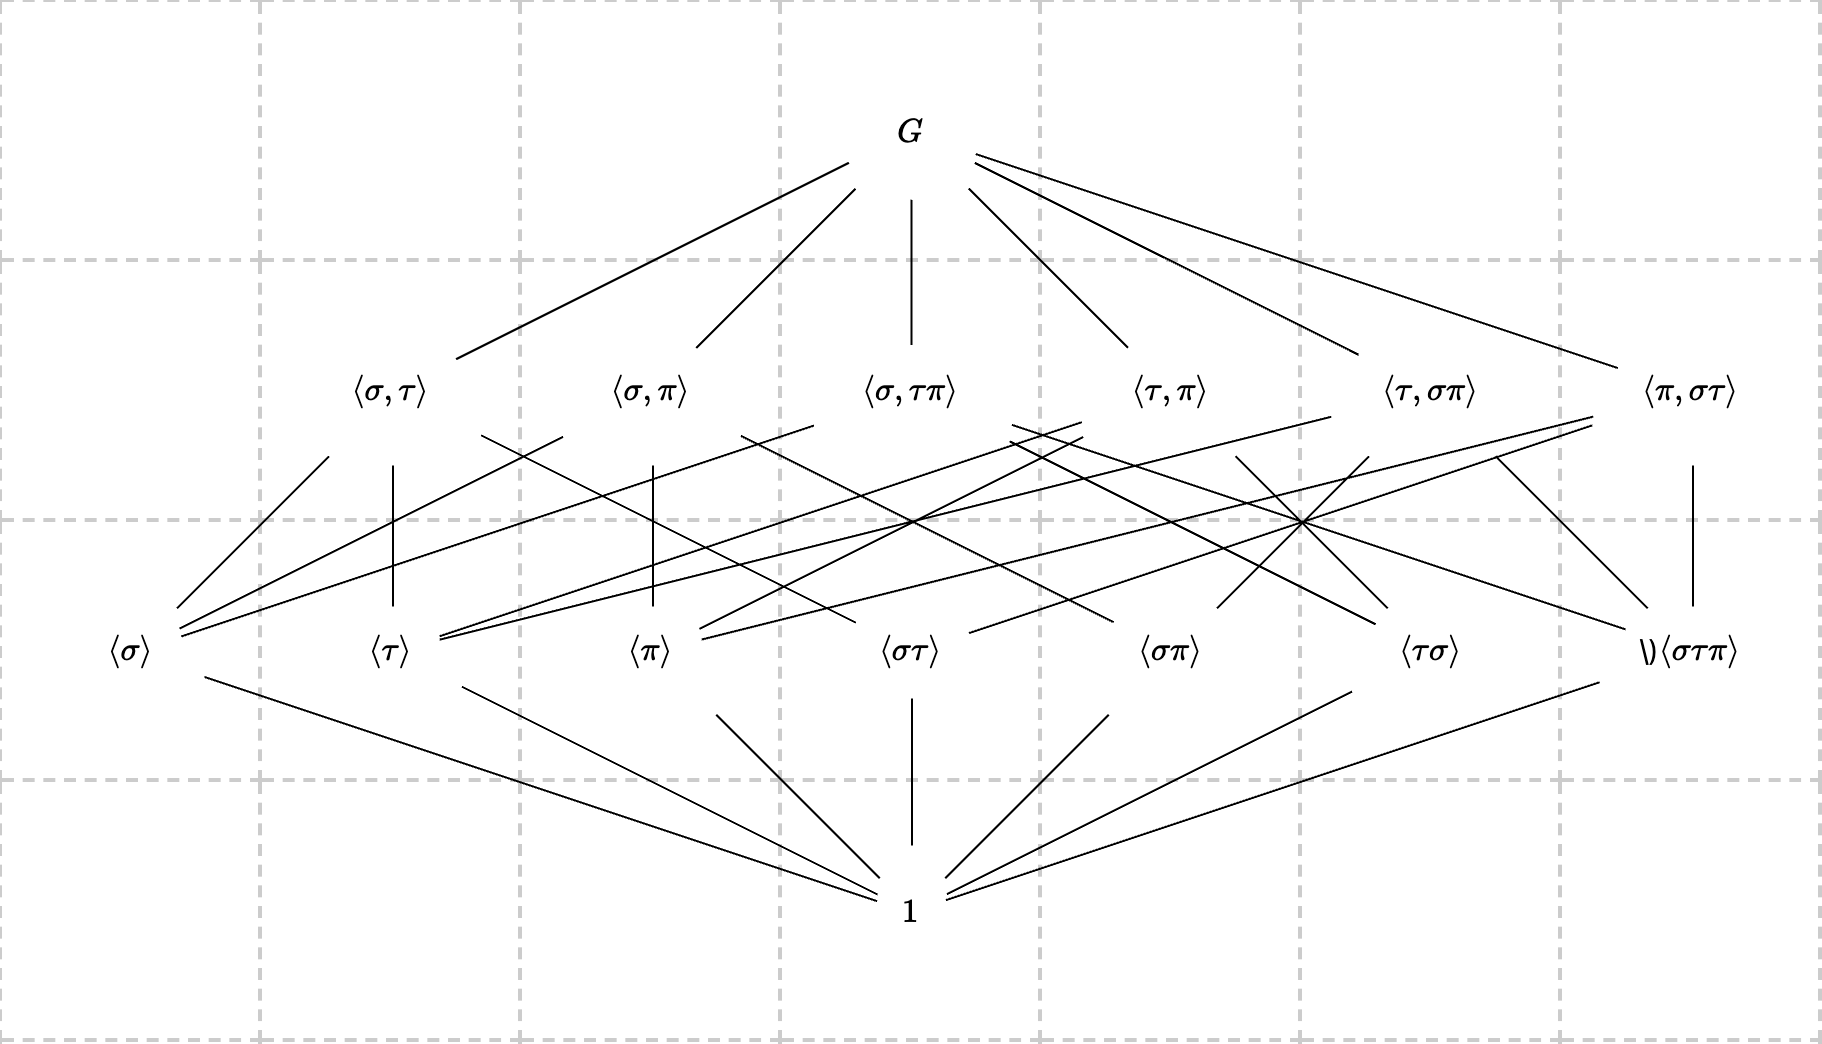
\includegraphics[scale=0.3]{fig/grp}
\end{figure}

And this yields the following (upside down) subfield lattice.
\begin{figure}[H]
	\centering
	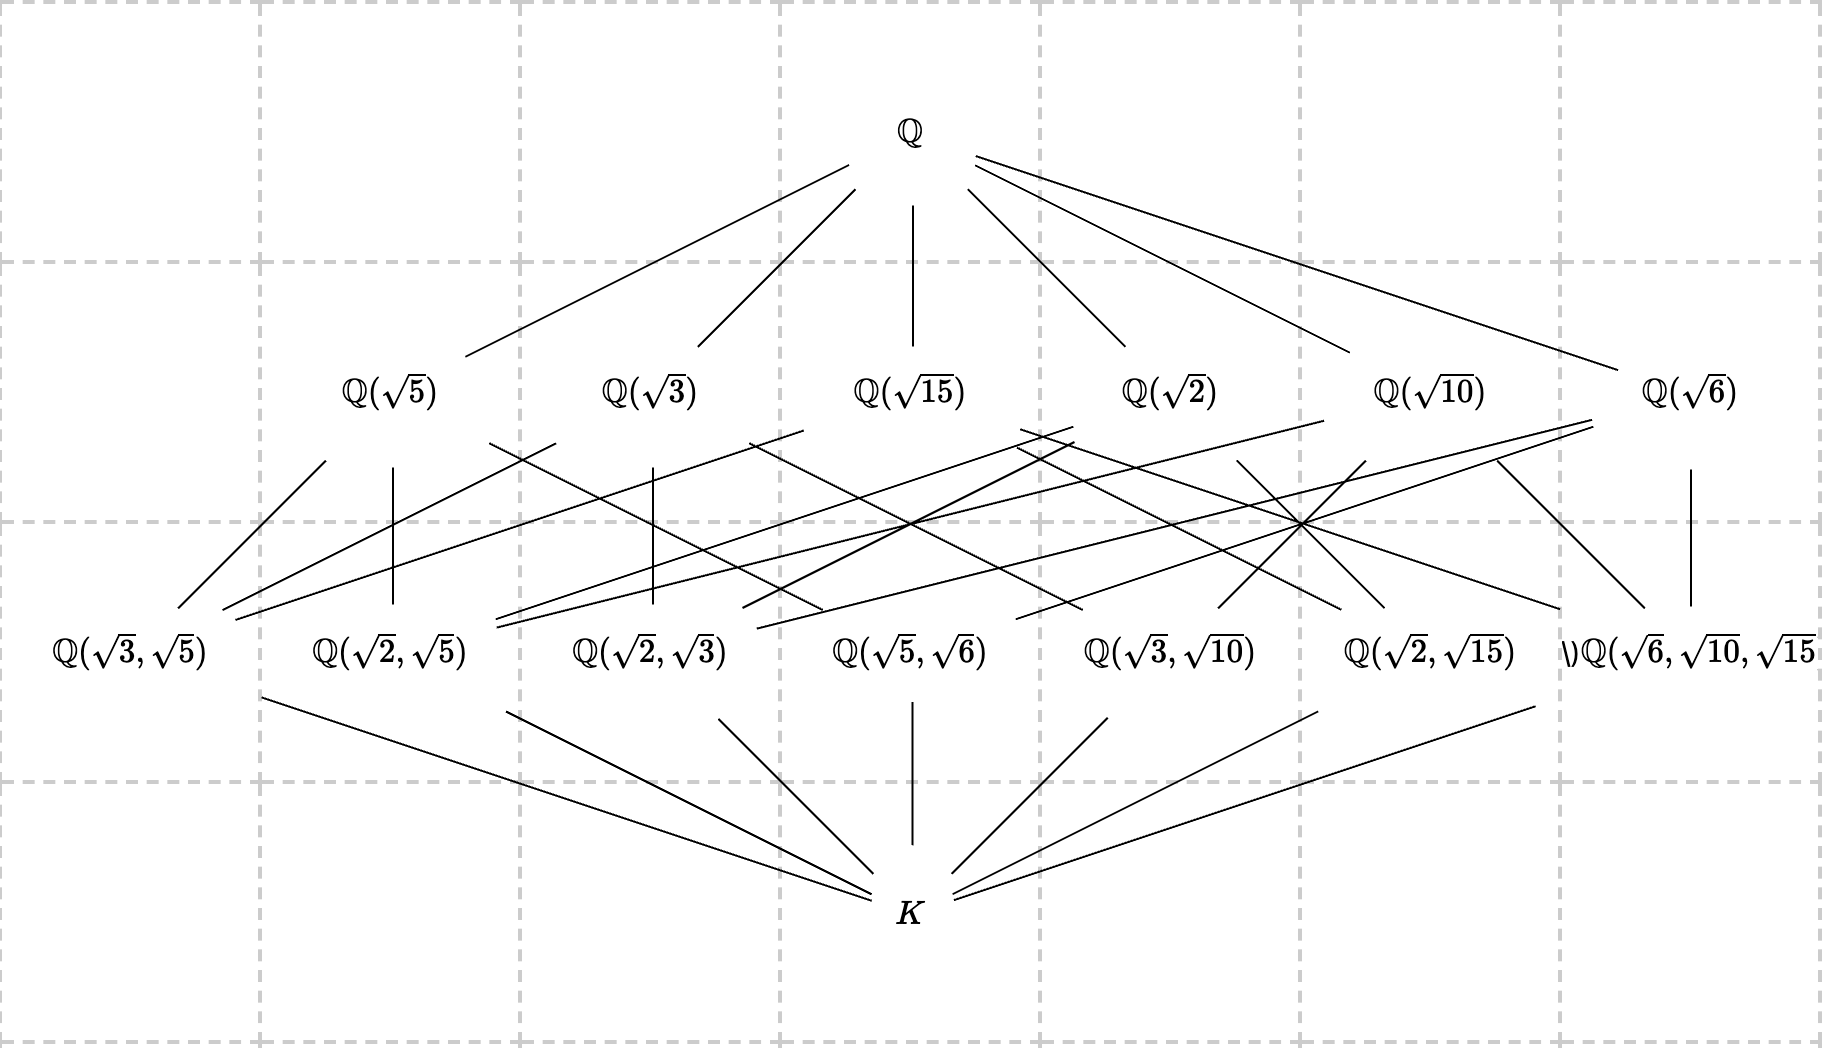
\includegraphics[scale=0.3]{fig/fld}
\end{figure}

\begin{exer}[DF 14.2: 6]
Show that $\text{Gal}_{F_1}(K)\cong Z_{8}$, $\text{Gal}_{F_2}(K)\cong D_{8}$, and $\text{Gal}_{F_3}(K)\cong Q_8$.
\end{exer}
By the example on DF page 577,
\[
G \doteq \text{Gal}_{\mathbb{Q}}(K)= \left\langle \sigma,\tau \;|\; \sigma^2 =\tau^2=1, \sigma\tau=\tau\sigma^3 \right\rangle,
\] where
\[
\sigma:
\begin{cases}
	\sqrt[8]{2} \mapsto \zeta_8 \sqrt[8]{2} \\
	i \mapsto i
\end{cases}, \quad
\begin{cases}
	\sqrt[8]{2} \mapsto \sqrt[8]{2} \\
	i \mapsto -i.
\end{cases}
\] Then by the Fundamental Theorem of Galois Theory, $\text{Gal}_{F_i}(K) \cong H_i / 1 = H_i$, where $H_i$ is the subgroup of $G$ that corresponds with $F_i$. By the diagrams on DF pages 580-581, we have the following correspondences:
\begin{align*}
	\mathbb{Q}(i) &\leftrightarrow \left\langle \sigma \right\rangle, \\
	\mathbb{Q}(\sqrt{2} ) &\leftrightarrow \left\langle \sigma \right\rangle, \\
	\mathbb{Q}(\sqrt{-2} ) &\leftrightarrow \left\langle \sigma^2, \tau \sigma^3 \right\rangle
\end{align*}

\begin{itemize}
	\item Now $\left\langle \sigma \right\rangle= \left\{ \sigma, \dots, \sigma^7, 1 \right\}$. If we denote 1 by $\sigma^0$, then the map $\sigma^k \mapsto k$ shows $\text{Gal}_{F_1}(K)\cong \left\langle \sigma \right\rangle\cong \mathbb{Z}_{8}$.
	\item DF defines $D_{2n} \doteq \left\langle r,s \;|\; r^n=s^2=1, rs=sr^{-1} \right\rangle$. By the definitions of $\sigma$ and $\tau$, we have $(\sigma^2)^4=\sigma^8=1$, $\tau^2=1$, and $\sigma^2\tau = \tau\sigma^6 = \tau (\sigma^2)^{-1}$. Then the map that sends $\sigma^2 \mapsto r$ and $\tau \mapsto s$ shows $\text{Gal}_{F_2}(K)\cong \left\langle \sigma^2, \tau \right\rangle\cong D_{8}$.
	\item DF defines $Q_8 = \left\{ 1,-1,i,-i,j,-j,k,-k \right\}$, where $i^2=j^2=k^2=1$ and
		\begin{align*}
			ij=k, &\quad ji=-k, \\
			jk=i, &\quad kj=-i, \\
			ki=j, &\quad ik=-j.
		\end{align*}
		Now $\left\langle \sigma^2,\tau\sigma^3 \right\rangle = \left\{ 1,\sigma^2,\sigma^4,\sigma^6,\tau\sigma,\tau\sigma^3,\tau\sigma^5,\tau\sigma^7 \right\}$. The map
		\begin{align*}
			1 &\mapsto 1 \\
			\sigma^2 &\mapsto i \\
			\sigma^4&\mapsto -1\\
			\sigma^6&\mapsto -i\\
			\tau\sigma&\mapsto k\\
			\tau\sigma^3&\mapsto j\\
			\tau\sigma^5&\mapsto -k\\
			\tau\sigma^7&\mapsto -j
		\end{align*}
		is then a bijection between $Q_8$ and $\left\langle \sigma^2,\tau\sigma^3 \right\rangle$, so $\text{Gal}_{F_3}(K) \cong \left\langle \sigma^2,\tau\sigma^3 \right\rangle \cong Q_8$.
\end{itemize}

\begin{exer}[14.2: 13]
	If the Galois group of the splitting field of a cubic over $\mathbb{Q}$ is the cyclic group of order 3, then all the roots of the cubic are real.
\end{exer}
Call the cubic $f$, and suppose that it does \textit{not} have all real roots. If $\alpha$ is one of the non-real roots, then its complex conjugate $\overline{\alpha} $ is also a root. Then the automorphisms over $Q$ are given by fixing $\alpha$ and sending $\alpha$ to $\overline{\alpha} $. Since the third root cannot have multiplicity greater than 1, any automorphism must fix it. Since there are only two automorphisms, the Galois group cannot possibly be the cyclic group of order 3, but this is a contradiction. Thus all the roots of $f$ must be real.

\begin{exer}[DF 14.3: 1]
Factor $x^8-x$ into irreducibles over $\mathbb{Z}$ and $\mathbb{F}_{2}$.
\end{exer}
\textbf{Over the integers:} 0 and 1 are clearly roots, and dividing $x^8-x$ by $x(x-1)$ gives $x^6 + x^5 + x^4 + x^3 + x^2 + x + 1$. But by the table on DF page 553, this is just $\Phi_{7}(x)$, so it is irreducible over $\mathbb{Z}$. Thus over $\mathbb{Z}$, $x^8-x$ factors into
\[
	x^8-x = x(x-1)(x^6 + x^5 + x^4 + x^3 + x^2 + x + 1).
\] 

\textbf{Over $\mathbb{F}_{2}$:} 0 and 1 are still roots, so we know that $x$ and $x-1=x+1$ will be factors of $x^8-x$. Unlike over $\mathbb{Z}$, it's possible to factor $x^6 + x^5 + x^4 + x^3 + x^2 + x + 1$ over $\mathbb{F}_{2}$ into $(x^3+x+1)(x^3+x^2+1)$. We know that $x^8-x = x^{2^3}-x$ is the product of all irreducible polynomials over $\mathbb{F}_{2}$ whose degrees divide $3$. Since only 1 and 3 divide 3, we know that we cannot reduce any further. Thus over $\mathbb{F}_{2}$,
\[
	x^8-x = x(x+1)(x^3+x+1)(x^3+x^2+1).
\] 

\begin{exer}[DF 14.3: 9]
\begin{enumerate}
	\item $\sigma_{q}$ fixes $\mathbb{F}_{q}$.
	\item Every degree $n$ extension of $\mathbb{F}_{q}$ is the splitting field of $x^q-x$ over $\mathbb{F}_{q}$, and hence is unique.
	\item Prove that every finite extension of $\mathbb{F}_{q}$ of degree $n$ is cyclic with $\sigma_{q}$ as generator.
	\item The subfields of the unique extension of $\mathbb{F}_{q}$ of degree $n$ are in bijective correspondence with the divisors $d$ of $n$.
\end{enumerate}
\end{exer}
\begin{enumerate}
	\item $\mathbb{F}_{q}$ is the splitting field of $x^q-x$, so $x \in \mathbb{F}_{q}$ satisfies $x^q-x=0$. Then $\sigma_{q}(x)=x^q=x$, so $\sigma_{q}$ fixes $\mathbb{F}_{q}$.
	\item Let $F$ denote a degree $n$ extension of $\mathbb{F}_{q}$, then $F$ is a finite field of order $p^{mn}=q^n$, so $F$ is the splitting field of $x^{p^{mn}}-x$ over $\mathbb{F}_{p}$ and thus also the splitting field of $x^{q^n}-x$ over $\mathbb{F}_{q}$. Thus $F$ is unique.
	\item By part (b), for all $x \in F$, $x^{q^n}=x$, so $\sigma_{q}^n=1$. For $k<n$, if $\sigma_{q}^k=1$, then $F$ is the splitting field of $x^{q^k}-x$. This is impossible, though, as $F$ has $q^n > q^k$ elements and $x^{q^k}-x$ has only $q^k$ total roots. Thus $\left\langle \sigma_{q} \right\rangle$ is of order $n$.

		We know that $\text{Gal}_{\mathbb{F}_{p}}(F)$ is cyclic of order $mn$ with generator $\sigma_{p}$, so since degrees multiply in towers, $G \doteq \text{Gal}_{\mathbb{F}_{q}}(F)$ has order $n$. By part (a), $\sigma_{q}$ fixes $\mathbb{F}_{q}$, so we know $\left\langle \sigma_{q} \right\rangle\leq G$. But since they both have order $n$, they must be equal. Thus $F$ is a cyclic extension of $\mathbb{F}_{q}$ with $\sigma_{q}$ as a generator.
	\item By the fundamental theorem of Galois theory, the subfields of $F$ are in bijective correspondence with the subgroups of $G = \text{Gal}_{\mathbb{F}_{q}}(F)$. By part (c), $G$ is cyclic or order $n$, so Langrange's theorem says that all subgroups of $G$ must have order dividing $n$. Thus the subfields of $F$ are in bijective correspondence with the divisors of $n$.
\end{enumerate}

\begin{exer}[]
Let $F$ be a field extension of $\mathbb{F}_{2}$ such that $|F| = 2^8$. Describe the Galois group $\text{Aut}_{\mathbb{F}_{2}}(F)$ and find all intermediate fields of the extension. Draw the subgroup and subfield lattices.
\end{exer}
$F$ is just $\mathbb{F}_{2^8}$, so its corresponding Galois group is generated by the Frobenius automorphism $\sigma_{2}: x \mapsto x^2$. Explicitly,
\[
\text{Aut}_{\mathbb{F}_{2}}(F) = \left\{ \sigma_2, \dots, \sigma_2^7, \sigma_{2}^8=1 \right\}.
\] The intermediate fields of $\mathbb{F}_{2^8}$ are the $\mathbb{F}_{2^d}$ with $d$ dividing $8$. The subgroup lattice will similarly be a tower with elements of the form $\langle \sigma_{2}^{8/d} \rangle$. Below are the subfield and subgroup lattices, with the subgroup lattice flipped upside down to show the proper correspondences with the subfields.

\begin{figure}[H]
	\centering
\begin{tikzcd}
	F=\mathbb{F}_{2^8} \arrow[d, no head] &  & \text{Aut}_{\mathbb{F}_{2}}F=\langle \sigma_2 \rangle \arrow[d, no head] \\
\mathbb{F}_{2^4} \arrow[d, no head]   &  & \langle \sigma_2^2 \rangle \arrow[d, no head]   \\
\mathbb{F}_{2^2} \arrow[d, no head]   &  & \langle \sigma_2^4 \rangle \arrow[d, no head]   \\
\mathbb{F}_{2}                        &  & 1 = \langle \sigma_2^8 \rangle
\end{tikzcd}

\end{figure}

\end{document}
